\chapter{Hiukkassuodatin}%
\label{ch:dpf}



Dieselmoottorin hiukkassuodatin, eli DPF (\emph{eng. Diesel Particulate Filter}) on tehokkain järjestelmä pakokaasun noki- ja tuhkapartikkeleiden suodatukseen. 
Hyvä DPF suodattaa läpivirtaavasta pakokaasusta jopa 99 \% hiukkaslukumäärästä ja 95 \% -massasta \cite{Yan_state_of_the_art}. Suodatetut hiukkaset ovat nokea ja hapettumatonta tuhkaa. Tässä työssä noen oletetaan koostuvan puhtaasta hiilestä. 



Tässä luvussa tarkastellaan hiukkassuodattimen toimintaa sekä fyysisenä järjestelmänä että matemaattisten mallien kautta. Luvussa esitellään noen massataseyhtälö ja siihen liittyvät regenerointi- ja painehäviöyhtälöt, joiden pohjalle työn estimointimenetelmä rakentuu.


\section{Jälkikäsittelyjärjestelmän fyysinen rakenne}
Moderni jälkikäsittelyjärjestelmä koostuu yleensä hapettavasta katalysaattorista (DOC, \emph{eng. Diesel Oxidation Catalyst}), hiukkassuodattimesta (DPF), sekä selektiivisestä katalyyttisestä pelkistimestä (SCR, \emph{eng. Selective Catalytic Reduction}). 
Jälkikäsittelyjärjestelmää on havainnollistettu Kuvassa \ref{fig:EAT_full}. %
%
\begin{figure}[H]
    \centering
    \pdftooltip{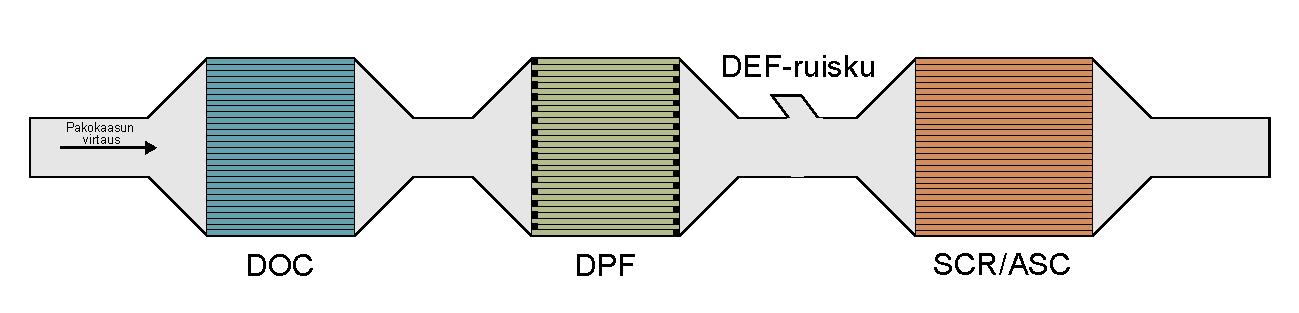
\includegraphics[width=\textwidth]{figures/EAT2.pdf}}
                {Kuvituskuva jälkikäsittelyjärjestelmästä. Kuvaan merkitty hapetuskatalysaattori, hiukkassuodatin ja selektiivinen katalyyttinen pelkistin.}
    \caption{Modernin jälkikäsittelyjärjestelmän osat.}
    \label{fig:EAT_full}
\end{figure}
%
Jälkikäsittelyjärjestelmän ensimmäinen osa on hapettava katalysaattori, eli DOC. 
Hapettavan katalysaattorin tehtävä on nimensä mukaan hapettaa moottorin raakapäästöjä, kuten hiilivetyjä, häkää ja typpimonoksidia \cite{dieselnet_doc}. Typpimonoksidista hapetettua typpidioksidia käytetään hiukkassuodattimessa noen hapettamiseen. 

Hapettavan katalysaattorin jälkeinen komponentti on hiukkassuodatin eli DPF.
Tyypillisin DPF-tyyppi on ns. seimämävirtaus-DPF (\emph{eng. wall-flow DPF}), jossa pakokaasu virtaa hunajakennomaisessa suodattimessa puoliavoimissa putkissa. Pakokaasu virtaa putkien välillä huokoisten seinämien läpi. Pakokaasun hiukkaset jäävät kiinni seinämien sisään ja pinnalle. Virtausta on havainnollistettu Kuvassa \ref{fig:wall-flow-dpf}.
%
\begin{figure}[H]
    \centering 
    \pdftooltip{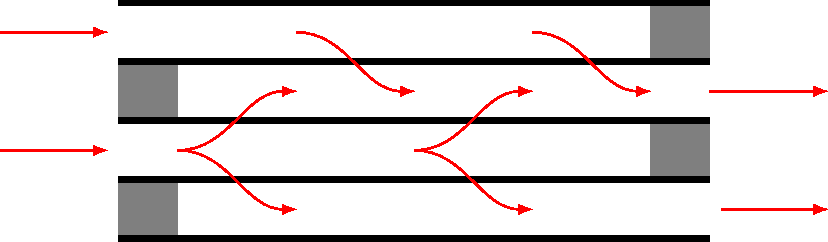
\includegraphics[width=\textwidth]{figures/wall_flow_DPF_figure.pdf}}
               {Kuvituskuva hiukkassuodattimen toiminnasta. Nuolilla kuvattu pakokaasu virtaa avoimiin putkiin ja kulkee seinämien läpi.}
    \caption{Pakokaasu virtaa suodattimessa huokoisten seinämien läpi. Yli 90 \% pakokaasun hiukkasmassasta jää huokoisten seinämien sisään ja pinnalle. Mukailtu lähteestä \cite{dieselnet_dpf}.}
    \label{fig:wall-flow-dpf}
\end{figure}
%
%Tässä työssä noen kerääntymistä seinämien sisään ja pinnalle ei erotella, vaan oletetaan nokimäärän kerääntyvän homogeeniseksi kerrokseksi.


Selektiivinen katalyyttinen pelkistin, eli SCR pelkistää ympäristölle ja terveydelle haitalliset typen oksidit typpikaasuksi ja vedeksi. Pelkistämiseen käytetään urealiuosta, josta käytetään nimitystä DEF (\emph{eng. Diesel Exhaust Fluid}) tai kauppanimeä AdBlue. Pelkistimen perässä on monesti vielä ammoniakin hapetuskatalysaattori (ASC, \emph{eng. Ammonia Slip Catalyst}), jolla voidaan hapettaa liikaruiskutettu ympäristölle ja terveydelle haitallinen DEF SCR-katalysaattorin poistovirtauksesta.
 \cite{dieselnet_scr}

Tässä työssä tarkastellaan jälkikäsittelyjärjestelmän komponenteista tarkemmin ainoastaan hiukkassuodatinta, vaikka DOC-katalysaattorin ulosvirtauksen typpidioksidikonsentraatio vaikuttaa DPF-järjestelmän regenerointiin. Typpidioksidikonsentraation mallin epävarmuuden vaikutusta DPF-tilan estimointimenetelmän varianssiin tutkitaan tarkemmin.



\section{Regenerointi}
Noen poistoa suodattimesta hapettamalla kutsutaan regeneroinniksi. Regenerointi jaetaan karkeasti kahteen tapaan: aktiiviseen ja passiiviseen regenerointiin. 
Aktiivinen regenerointi tarkoittaa käytännössä noen polttamista ja se
vaatii korkean, yli 600:n \degree C lämpötilan. Tarvittava energia saadaan ajoneuvon polttoainetta käyttämällä \cite{dieselnet_dpf}. Passiiviseen regenerointiin riittää huomattavasti matalammat lämpötilat ja se perustuu noen hapetusreaktioihin typpidioksidin (NO\(_2\)) kanssa. Tarvittava typpidioksidi saadaan hapettamalla moottorin raakapäästöinä muodostuvaa typpimonoksidia (\ce{NO}) hapettavassa katalysaattorissa (DOC, \emph{Diesel Oxidation Catalyst}).

Regeneroidessa tapahtuvat reaktiot ovat  
\begin{align}
    \ce{C + 1/2 O2 &->[$R_1$] CO }\label{req:active1}\\
    \ce{C + O2 &->[$R_2$] CO2}\label{req:active2}\\
    \ce{C + NO2 &->[$R_3$] CO +  NO} \text{ ja }  \label{req:passive1} \\
    \ce{C + 2 NO2 &->[$R_4$] CO2 + 2 NO}. \label{req:passive2}
    % \\\ce{NO + 1/2 O2 &<=>[$R_5$] NO2}.
\end{align}
Niiden reaktionopeudet voidaan määrittää Arrheniuksen yhtälöinä \cite{LiuGuanlin2021Roio} \cite{Penghao_regen}
\begin{align}
    R_i =  k_i \exp\left({-\frac{E_{a,i}}{RT}}\right),\ i = 1,\ldots,4
\end{align}
jossa \(k_i\) on reaktion \(i\) frekvenssitekijä, \(E_{a, i}\) on  reaktion \(i\)aktivoitumisenergia, \(R\) on moolinen kaasuvakio ja \(T\) on lämpötila. Karkeasti jaoteltuna reaktiot \eqref{req:active1} ja \eqref{req:active2} kuvaavat aktiivista regenerointia, ja vastaavasti reaktiot \eqref{req:passive1} ja \eqref{req:passive2} passiivista regenerointia.
Suodattimessa tapahtuu paljon muitakin reaktioita \cite{Penghao_regen}, mutta ne eivät ole tämän työn kannalta olennaisia.
Reaktionopeus kuvaa kunkin aineen konsentraation muutosnopeutta, eli aikaderivaattaa \cite[s. 24-26]{chemical_reaction_kinetics}. Suljetulle reaktiolle
\begin{align}
    \ce{a1 X1 + a2 X2 + \cdots {} + a_n X_n ->[R] b1 Y1 + b2 Y2 + \cdots {} + b_m Y_m}
\end{align}
reaktionopeus \(R\) määritellään
\begin{align}
    R   = -\frac{1}{\ce{a1}}\frac{d[\ce{X1}]}{dt} 
        % = -\frac{1}{\ce{a2}}\frac{d[\ce{X2}]}{dt}
        = \cdots 
        = -\frac{1}{\ce{a_n}}\frac{d[\ce{X_n}]}{dt}
        = \frac{1}{\ce{b1}}\frac{d[\ce{Y1}]}{dt} 
        = \cdots 
        = \frac{1}{\ce{b_m}}\frac{d[\ce{Y_m}]}{dt},
\end{align}
jossa \(\ce{[X_i], [Y_i]}\) on aineiden \(\ce{X_i, Y_i}\) konsentraatiot. 

% Noen regeneroitumista reaktioissa \eqref{req:active1} ja \eqref{req:active2} kuvaa massataseyhtälö \cite{BaiShuzhan2016Slem} \cite{ZhongChao2022Eaos}
% \begin{align}
%     \frac{d m_{soot}}{dt}\Big |_{[\ce{NO2}]} = (R_1 + R_2) m_{soot}^\gamma,
% \end{align}
% ja reaktioissa \eqref{req:passive1} ja \eqref{req:passive2} massataseyhtälö 
% \begin{align}
%     \frac{d m_{soot}}{dt}\Big |_{[\ce{O2}]} = (R_3 + R_4) m_{soot}^\gamma [\ce{NO2}]^\alpha.
% \end{align}
% Taseyhtälöissä \(m_{soot}\) on suodattimeen kertyneen noen massa, \(R_i\) on reaktionopeus, ja \(\alpha\) ja \(\gamma\) ovat noen massaan ja typpidioksidin konsentraatioon liittyvät parametrit.


Aktiivisen regeneroinnin reaktionopeudet voidaan kirjoittaa muodossa
\begin{align}
    R_1 &= f_{\ce{CO}} k_1 \exp{\left( \frac{E_{a, 1}}{RT} \right)} \\% [\ce{O2}] \\
    R_2 &= (1-f_{\ce{CO}}) k_1 \exp{\left( \frac{E_{a, 1}}{RT} \right)} ,%[\ce{O2}],
\end{align}
ja vastaavasti passiivisen regeneroinnin reaktionopeudet voidaan kirjoittaa muodossa
\begin{align}
    R_3 &= f_{\ce{NO}} k_2 \exp{\left( \frac{E_{a, 2}}{RT} \right)} \\%[\ce{NO2}], \\
    R_4 &= (1-f_{\ce{NO}}) k_2 \exp{\left( \frac{E_{a, 2}}{RT} \right)}, % [\ce{NO2}],
\end{align}
joissa \( f_{\ce{CO}}\) ja \( f_{\ce{NO}}\) ovat reaktioiden selektiivisyyteen liittyvät termit \cite{ZhongChao2022Eaos} \cite{DengYuanwang2017Iogc}.
Kaasujen konsetraatiot hiukkassuodattimessa ovat paikan suhteen vakioita, joten työssä voidaan tarkastella vain aktiiviseksi ja passiiviseksi reaktioksi yksinkertaistettuja reaktioita.
Näin ollen regenerointien kokonaisreaktionopeudet ovat
\begin{align}
    R_{active} &= R_1 + R_2 =   k_1 \exp{\left( \frac{E_{a, 1}}{RT} \right)} \\%[\ce{O2}], \\ \text{ ja }
    R_{passive} &= R_3+ R_4 =  k_2 \exp{\left( \frac{E_{a, 2}}{RT} \right)} . %[\ce{NO2}].
\end{align}

% Tästä eteenpäin ei fco, fno

Hiukkassuodattimen nokimäärän massataseyhtälö on tällöin
\begin{align}
    \frac{dm_{soot}}{dt} = m_{soot, in} - m_{soot, oxi}
    =m_{soot, in} - m_{soot} \left( R_{active}[\ce{O2}] + R_{passive}[\ce{NO2}] \right),
\end{align}
jossa \(m_{soot}\) on suodattimeen kertyneen noen massa.


\section{Painehäviö ja sen mallintaminen}
Hiukkassuodattimeen kertyneiden hiukkasten lukumäärää arvioidaan painehäviön avulla. Painehäviötä voidaan mitata hiukkassuodattimen yli paineantureilla, mutta olennaisesti noen ja tuhkan määrän arvointiin tarvitaan matemaattinen malli.
Konstandopoulos et al. esittelevät artikkelissaan \cite{Konstandopoulos2000} symmetrisen, nokilatautuneen hiukkassuodattimen painehäviömallin. Tässä työssä tarkastellaan yleisesti epäsymmetristä suodatinta ja laajennetaan mallia ottamaan huomioon myös tuhka. Toisin sanoen tarkastellaan tilannetta, jossa sisäänmeno- ja ulostulokanavien poikkipinta-alat voivat olla eri kokoisia. Lisäksi kokonaispainehäviömalliin otetaan mukaan myös tuhkakerroksen aiheuttama painehäviö. Näin ollen kokonaispainehäviö on puhtaan suodattimen sisäänmenon, ulostulon ja seinämien, sekä noki- ja tuhkakerrosten aiheuttamien painehäviöiden summa \cite{Konstandopoulos2000}\cite{Konstandopoulos2008}, eli
\begin{align}
    \Delta P_{tot} = \Delta P_{inlet} +  \Delta P_{outlet} + \Delta P_{wall} + \Delta P_{soot} +  \Delta P_{ash}.
\end{align}
Lisäksi painehäviötä tapahtuu sisäänmeno- ja ulostuloaukolla, mutta häviöt näissä ovat merkityksettömän pieniä \cite{Konstandopoulos2000}.
% Tilavuusvirtaus saadaan massavirrasta ja tiheydestä
% \begin{align}
%     Q(t,T) = \frac{\dot{m}(t)}{\rho(T)}.
% \end{align}

Tarkastellaan aluksi puhdasta suodatinta. Puhtaassa suodattimessa yhden kanavan painehäviö on
\begin{align}
    \Delta P_{channel} = \frac{\mu F}{3 \alpha^2} LU_{channel},
\end{align}
jossa \(\mu \) on pakokaasun viskositeetti, \(F\) on kanavien kitkaan liittyvä kerroin \cite{dieselnet_wall_flow_monolith}, \(\alpha\) on kanavan leveys, \(L\) on kanavan pituus ja \(U_{channel}\) on virtausnopeus \cite{Konstandopoulos2000}.
Muokataan yhtälöä hyödyntäen sylinterin geometriaa. Kun merkitään \(\frac{1}{A} = \frac{L}{V}\), jossa \(A\) on suodattimen poikkileikkauspinta-ala ja \(V\) on suodattimen kokonaistilavuus, painehäviö voidaan esittää muodossa
\begin{align}\label{eq:clean_channel_pd}
    \Delta P_{channel} = \frac{\mu F}{3 \alpha^2} \frac{L^2}{V}U_{channel},
\end{align}

Yleisesti suodattimen sisäänmeno- ja ulostulokanavien leveydet \(\alpha_{in}\) ja \(\alpha_{out}\) eivät ole identtiset. Toisin sanoen \(\alpha_{in} \neq \alpha_{out}\). Tällaista suodatinta on havainnollistettu Kuvassa \ref{fig:hac_dpf_clean}.
%
\begin{figure}[H]
    \centering 
    \pdftooltip{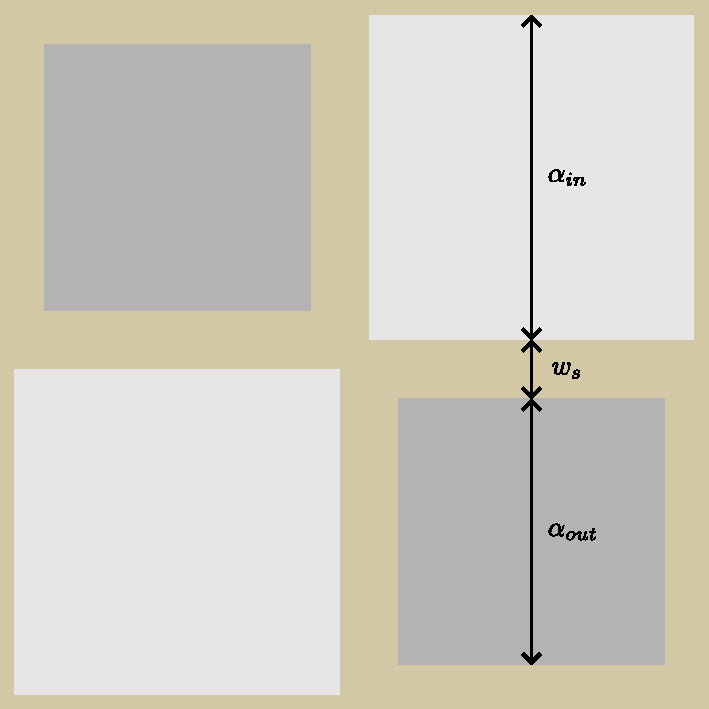
\includegraphics[width=0.6\textwidth]{figures/dpf_clean_new.pdf}}
               {Poikkileikkauskuva neljästä DPF-solusta. Kuvassa menokanavat ovat suuremmat kuin ulostulokanavat.}
    \caption{DPF-poikkileikkaus neljästä solusta. Sisäänmeno- ja ulostulokanavien leveydet eivät ole välttämättä samat. Havainnollistuksessa \(\alpha_{in}>\alpha_{out}\).}
    \label{fig:hac_dpf_clean}
\end{figure}

Yhden puhtaan suodatinkanavan sisäänmenonvirtausnopeus määritellään 
\begin{align}\label{eq:flow_velocity_clean}
    U_{channel} = \frac{Q}{A_{cell}},
\end{align}
jossa \(Q\) on tilavuusvirtaus ja \(A_{cell}\) on  yhden solun poikkipinta-ala ja suodattimen sisäänmenon efektiivinen pinta-ala \cite{Konstandopoulos2000}. Solulla tarkoitetaan kanavan ja seinämän muodostamaa kokonaisuutta, ja sen pinta-ala on Kuvan \ref{fig:hac_dpf_clean}  geometriaan nojaten
\begin{align}
    A_{cell}=\frac{1}{4}(\alpha_{in}+\alpha_{out}+2w_s)^2.
\end{align}

Kokonaisvirtausnopeudet saadaan sisäänmenon ja ulostulon solujen pinta-alan avulla
\begin{align}
    A_{eff, in} &= 2 \pi \left(\frac{D}{2}\right)^2 \cdot \frac{\alpha_{in}^2}{(\alpha_{in}+\alpha_{out}+2w_s)^2}, \label{eq:area_eff_in} \\
    A_{eff, out} &= 2 \pi \left(\frac{D}{2}\right)^2 \cdot \frac{\alpha_{out}^2}{(\alpha_{in}+\alpha_{out}+2w_s)^2},\label{eq:area_eff_out}
\end{align}
jossa \(D \) suodattimen halkaisija, ja kerroin \(\frac{1}{2}\) poistaa efektiivisestä pinta-alasta suljetut kanavat.

Sisäänmenon ja ulostulon virtausnopeudet ovat tällöin
\begin{align}
    U_{in} &= \frac{Q}{A_{eff, in}}, \label{eq:uin}\\
    U_{out} &= \frac{Q}{A_{eff, out}}. \label{eq:uout}
\end{align}

Sijoittamalla yhtälöt \eqref{eq:uin} ja \eqref{eq:area_eff_in}, sekä \eqref{eq:uout} ja \eqref{eq:area_eff_out} yhtälöön \eqref{eq:clean_channel_pd} saadaan
\begin{align}
    \Delta P_{inlet} &=\frac{Q \mu F}{6}\cdot \frac{L^2}{V} \cdot \frac{(\alpha_{in}+\alpha_{out}+2w_s)^2}{\alpha_{in}^4} \label{eq:DeltaP_inlet_clean}
    \\ 
    \Delta P_{outlet} &=\frac{Q \mu F}{6}\cdot \frac{L^2}{V} \cdot \frac{(\alpha_{in}+\alpha_{out}+2w_s)^2}{\alpha_{out}^4}.
\end{align}
Jos kanavat ovat keskenään saman kokoiset, eli  \(\alpha_{in}=\alpha_{out}=\alpha\), saadaan sisäänmeno- ja ulostulokanavien painehäviöiksi 
\begin{align}
    \Delta P_{inlet}= \Delta P_{outlet} =  \frac{Q\mu F}{3} \frac{L^2}{V}\frac{(\alpha+w_s)^2}{\alpha^2}.
\end{align}


Kanavien lisäksi painehäviötä tapahtuu seinämissä. Seinämien painehäviötä mallinnetaan usein Darcyn lailla \cite{dieselnet_wall_flow_monolith}\cite{Konstandopoulos1989_wallflow}
\begin{align}
    q = - \frac{\kappa}{\mu}\nabla P,
\end{align}
jossa \(q\) on Darcyn nopeus, \(\kappa\) on väliaineen permeabiliteetti ja \(\nabla P\) on painegradientti \cite{feder2021_porous}. 
 Darcyn nopeus on vuo \cite{reible_env_eng}, joka kuvaa tilavuusvirtausta pinnan läpi. Näin ollen saadaan yhtälö
\begin{align}
    Q = \int_A q \cdot dA = \int_A - \frac{\kappa}{\mu} \nabla P \cdot dA.
\end{align}
Pakokaasun oletetaan kulkevan seinämän läpi kohtisuoraan, joten painehäviö voidaan laskea yksiulotteisesti. Kun valitaan suunnan merkiksi \(x\) saadaan
\begin{align}
    Q = - \frac{\kappa}{\mu} \frac{dP}{dx} \int_A dA = - \frac{\kappa}{\mu} \frac{dP}{dx} A.
\end{align}
Kun \(dx \to w_s\), niin \(dP \to -\Delta P_{wall}\). Näin ollen painehäviö on
\begin{align}
    \Delta P_{wall} = Q\mu \frac{w_s}{\kappa}.
\end{align}
Suodattimessa on jokaista sisäänmenokanavaa kohden neljä seinämää, ja avoimia kanavia on yhteensä \(n_{open}\) kappaletta. Yhden seinämän pinta-ala on \(L\cdot \alpha_{out}\), joten 
\begin{align}
    A = 4 n_{open} L \alpha_{out}.
\end{align}
Seinien kokonaispainehäviö on
\begin{align}
    \Delta P_{wall} =  Q \mu \frac{w_s}{4 n_{open} L  \alpha_{out}  \kappa_{wall}}.
\end{align}

Tarkastellaan nyt partikkelilatautunutta suodatinta.
Kertyneet noki ja tuhka mallinnetaan erillisiksi kerroksiksi suodattimen sisäänmenokanavissa. Kerrosten paksuudet voidaan  olettaa yhtenäisiksi \cite{Konstandopoulos2000}, sillä virtaus pyrkii aina kulkemaan pienimmän vastuksen reittiä. Kuvassa \ref{fig:hac_dpf_loaded} on havainnollistettu noki- ja tuhkakerrosta suodattimen sisäänmenokanavissa.
\begin{figure}[H]
    \centering 
    \pdftooltip{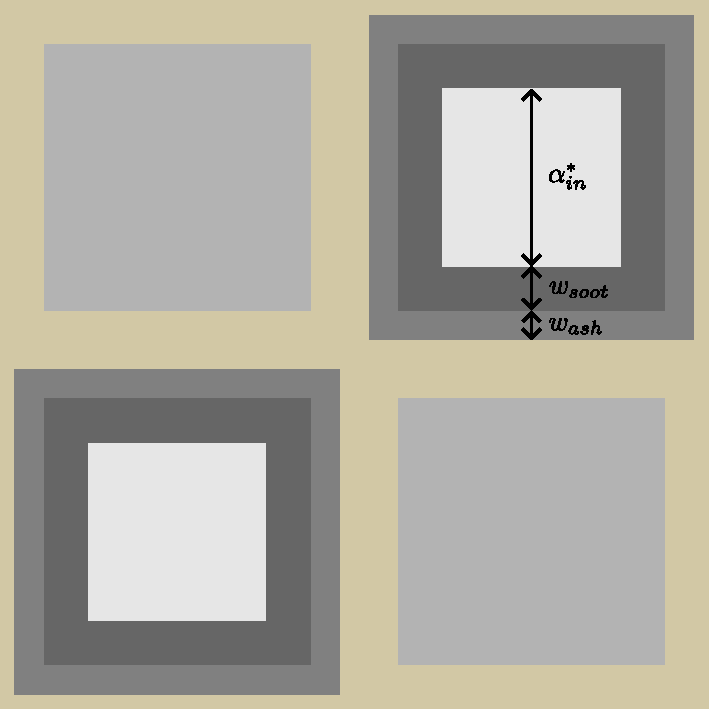
\includegraphics[width=0.6\textwidth]{figures/dpf_loaded_new.pdf}}
               {Kuvituskuva neljästä DPF-solusta. Sisäänmenokanavien reunoilla on kerros tuhkaa ja nokea.}
    \caption{Noki- ja tuhkalatautunut DPF. Sisäänmenokanavan efektiivinen leveys on pienempi, mikä täytyy ottaa mallissa huomioon.}
    \label{fig:hac_dpf_loaded}
\end{figure}
Noki- ja tuhkakerroksen paksuuksia merkitään \(w_{soot}\) ja \(w_{ash}\).
Koska noki ja tuhka kertyvät mallissa tasaisesti sisäänmenokanavien seinämille, tulee partikkelikerrokset ottaa huomioon sisäänmenon painehäviöyhtälössä \eqref{eq:DeltaP_inlet_clean}. Uusi sisäänmenokanavan leveys on 
\begin{align}
    \alpha_{in}^* = \alpha_{in} -2w_{soot}-2w_{ash}.
\end{align}
Näin ollen saadaan suodattimen sisäänmenon painehäviö
\begin{align}
    \Delta P_{inlet} = \frac{Q \mu F}{6}\cdot \frac{L^2}{V} \cdot \frac{(\alpha_{in}+\alpha_{out}+2 w_s)^2}{(\alpha_{in}^*)^4}.
    \label{eq:PDinletchannel}
\end{align}
Seinämien ja ulostulon painehäviöihin noki- ja tuhka eivät vaikuta. 
Tarkastellaan vielä noki- ja tuhkakerroksen aiheuttamia painehäviöitä. Molemmat kerrokset ovat huokoisia, joten niiden aiheuttamat painehäviöt voidaan mallintaa keskenään samalla tavalla. Nokikerroksen painehäviö saadaan \cite{Konstandopoulos2000} mukaan laskettua integroimalla Darcyn lakia partikkelikerroksen läpi. Laajennetaan mallia myös tuhkakerrokselle. Oletetaan mallissa kaiken tuhkan olevan seinämää lähempi kerros, ja vastaavasti kaiken noen olevan tuhkakerroksen päällä.
Tuhkakerroksen painehäviö on
\begin{align}
    \Delta P_{ash} &= \frac{\mu}{\kappa_{ash}} \int_0^{w_{ash}}  \frac{Q}{A}dx 
    \nonumber\\ &= \frac{Q \mu }{4 n_{open} L \kappa_{ash}} \int_0^{w_{ash}}  \frac{1}{\alpha_{out}-2w_{ash}+2x}dx 
    \nonumber \\ &= \frac{Q\mu}{8 n_{open} L \kappa_{ash}}\ln\left(\frac{\alpha_{out}}{\alpha_{out}-2w_{ash}}\right).
\end{align}
vastaavasti nokikerroksen painehäviö voidaan laskea integroimalla Darcyn lakia. 
\begin{align}
    \Delta P_{soot }&= \frac{\mu}{\kappa_{soot}} \int_{0}^{w_{soot}}  \frac{Q}{A}dx 
    \nonumber\\    &= \frac{Q \mu }{4 n_{open} L \kappa_{soot}} \int_{0}^{w_{soot}}  \frac{1}{\alpha_{out}-2w_{ash}-2w_{soot}+2x}dx 
    \nonumber \\ &= \frac{Q\mu}{8 n_{open} L \kappa_{soot}}\ln\left(\frac{\alpha_{out}-2w_{ash}}{\alpha_{out}-2w_{ash}-2w_{soot}}\right).
\end{align}

Tuhkakerroksen paksuus saadaan kaavalla
\begin{align}
    w_{ash} = \frac{\alpha_{in} - \sqrt{\alpha_{in}^2 - \frac{m_{ash}}{ n_{open} L \rho_{ash}}}}{2},
\end{align}
ja nokikerroksen paksuus vastaavasti kaavalla
\begin{align}
    w_{soot}= \frac{\alpha_{in}-2w_{ash} - \sqrt{(\alpha_{in}-2w_{ash})^2 - \frac{m_{soot}}{ n_{open} L \rho_{soot}}}}{2}.
\end{align}